% * * * * * * * * * * * * * * * * * * * * * * * * * * * * * * * * * * *
% *                             Thesis                                *
% *                 https://github.com/Jacopx/Thesis                  *
% * * * * * * * * * * * * * * * * * * * * * * * * * * * * * * * * * * *

\documentclass[%
    corpo=12pt,
    twoside,
%    stile=classica,
    oldstyle,
    autoretitolo,
    greek,
    evenboxes,
%    tipotesi,
]{toptesi}
%%%%%%%%%%%%%%%%%%%%%%%%%%%%%%%%%%%%%%%%%%%%%%%%%%%%

\usepackage[utf8]{inputenc}
\usepackage[T1]{fontenc}
\usepackage{lmodern}
\usepackage{hyperref}
\usepackage{graphicx}
\usepackage{subfigure}
\usepackage{booktabs}
\usepackage{amsfonts}
\usepackage{amsmath}
\usepackage{amssymb}
\usepackage{bm}
\usepackage{listings}

\hypersetup{%
    pdfpagemode={UseOutlines},
    bookmarksopen,
    pdfstartview={FitH},
    colorlinks,
    linkcolor={blue},
    citecolor={blue},
    urlcolor={blue}
  }

%%%%%%% Definizioni locali

\interlinea{1.5} 


\begin{document}

\ateneo{Politecnico di Torino}
%
% Non tutte le università hanno un nome proprio
%\nomeateneo{Sede di Torre Elettra}
%
% \FacoltaDi{Faculty of Computer Engineering}% lo spazio finale correttamente sparisce

\titolo{Defect prediction in software development via machine learning}
\sottotitolo{Artificial Intelligence applied to Software Engineering}

%
%%%%%%% Corso degli studi
\corsodilaurea{Computer Engineering}% per la laurea
%\corsodidottorato{Meccanica}% per il dottorato

\renewcommand*\IDlabel{}
%
\candidato{Jacopo \textsc{Nasi} [255320]}

%%%%%%% Relatori o supervisori
\relatore{prof.~Maurizio \textsc{Morisio}}

%%%%%%% Tutore
\tutoreaziendale{dott.\ Davide \textsc{Piagneri}}

\sedutadilaurea{\textsc{April} 2020}


%%%%%%% Logo della sede
\logosede{polito}

%%%%%%% OFFSET
%\setbindingcorrection{3mm}

\english%  di default e' in vigore \italiano

\iflanguage{english}{%
	\retrofrontespizio{This work is subject to the Creative Commons Licence}
	\DottoratoIn{PhD Course in\space}
	\CorsoDiLaureaIn{Master degree course in\space}
	\NomeMonografia{Bachelor Degree Final Work}
	\TesiDiLaurea{Master Degree Thesis}
	\NomeDissertazione{PhD Dissertation}
	\InName{in}
	\CandidateName{Candidates}% or Candidate
	\AdvisorName{Supervisors}% or Supervisor
	\TutorName{Tutor}
	\NomeTutoreAziendale{Internship Tutor}
	\CycleName{cycle}
	\NomePrimoTomo{First volume}
	\NomeSecondoTomo{Second Volume}
	\NomeTerzoTomo{Third Volume}
	\NomeQuartoTomo{Fourth Volume}
	\logosede{polito}% or comma separated list of logos
}{}
%%%%%%%%%%%%%%%%%%%%%%%%%%%%%%%%%%%%%%%%%

\frontespizio
\summary
Every day thousands of commit are pushed, each one contains a lot of information: files changed, changes, comments, test log and even more. A structured and correctly managed sourcing control allows the extraction of useful data that can be analysed using artificial intelligence.\\
To be able to use the data, some preliminary steps are necessary: the first step aim to study the structure of the data to allow the extraction of more information, next the data must be pre-processed to remove outliers and not useful features, with a clean dataset the extraction of combined data begin, information like developer seniority, bag of words of modified components, release version and other potentially useful information. The final step is the weekly aggregation by computing the difference between the closed and opened issues, translating the priority label to a value extracted from the duration distribution of the different classes. Once extracted the data can be passed through artificial intelligence models: Random Forest, Gradient Boosting and Neural Networks, to be forecasted with different time horizons. The evaluation can be performed in different ways: train-test over single extraction, cross-version, and even cross-project.\\
The execution with the best performance is the cross-project one, with a precision greater than 90\% up to 4 weeks and still greater than 70\% up to 20 weeks.


\acknowledgements

Un ringraziamento speciale a Smirnuff ed i suoi cavalieri, luce della mia battaglia.

\indici

\mainmatter

% #######################################
% #            Introduction             #
% #######################################

\chapter{Introduction}
\label{chap:intro}
\section{General Problem}
The software development is fundamental in the new world, how about using artificial intelligence to improve it?\\
The development of a software product is not different from any kind of hardware product development, after the first phase of design the production starts, during it problems emerge systematically and must be managed before the release in production.\\
Every day each a software house performs hundreds of commit, each one contains a lot of information linked to an issue, with structured commit, driven issue report and other software engineering stuff, the quality of the sourcing improves, allowing data to be used in artificial intelligence analysis. Predicting defectiveness during the making of the software can drastically improve the process of development, allocating the correct number of developers could reduce the time required and avoid delays and problems before releases.
With a correct preprocessing and evaluated aggregation, neural networks can predict, with high accuracy, the defectiveness trend. These forecast can be further used to improve the software engineering background of the related project.\\
Forecasting is one of the most critic part of a company, it could drive to easily success as well as drive to failure.
The software development experience shows that the process of analysis is really difficult, due to the nature of the problem, coding is a mind product and the time required to produce it can varying in accordance with a lot of different factors.

\section{Tools used}
This work is mainly conducted using software tools, here a list of the tools used:

\paragraph{\href{https://www.python.org/}{Python}} The main programming language of the thesis project. Used for data management, feature extraction, machine learning models and for interfaction with other softwares. The specific version used is the v3.7.0

\paragraph{\href{https://pandas.pydata.org/}{Pandas}} Open source, BSD-licensed library providing high-performance, easy-to-use data structures and data analysis tools for the Python programming language.

\paragraph{\href{https://numpy.org/}{NumPy}} Scientific computing with Python.

\paragraph{\href{https://matplotlib.org/}{Matplotlib}} 2D Plotting library for Python.

\paragraph{\href{https://seaborn.pydata.org/}{Seaborn}} Another plotting library for Python.

\paragraph{\href{https://www.tensorflow.org/}{Tensorflow}} Platform for machine learning.

\paragraph{\href{https://keras.io/}{Keras}} High level API for neural networks.

\paragraph{\href{https://scikit-learn.org/stable/}{SciKit-Learn}} Tools and libraries for machine learning.

\paragraph{\href{https://gitlab.com}{GitLab}} Sourcing platform based on Git. Used for the code of the project.
% \url{https://gitlab.com/EiS-Projects/analytics/temp/thesisProjectJN}.

\paragraph{\href{https://github.com}{GitHub}} Sourcing platform based on Git. Used for the thesis and calendar sourcing:
\begin{itemize}
  \item Thesis: \url{https://github.com/Jacopx/Thesis}
  \item Calendar: \url{https://github.com/Jacopx/ThesisCalendar}
\end{itemize}

\paragraph{\href{https://www.jetbrains.com/}{JetBrains IDEs}} Student-free IDE for different language development, product used:
\begin{itemize}
  \item PyCharm: \url{https://www.jetbrains.com/pycharm/}
  \item DataGrip: \url{https://www.jetbrains.com/datagrip/}
\end{itemize}

% #######################################
% #            State of art             #
% #######################################
\chapter{State of art}
\section{Related works}
Speaking about other works.

% #######################################
% #              Datasets               #
% #######################################

\chapter{Datasets}
\label{chap:dataset}
The following section illustrates the structure of all the principal datasets used during this thesis project.
\section{SEOSS33}
The SEOSS33\cite{SEOSS33} is a \href{https://doi.org/10.7910/DVN/PDDZ4Q}{dataset} collecting bug, issue, reports, commit and a lot of other information of 33 open source project, following their progress via sourcing platform. The dataset is enriched also with timestamps, release versions, component information, and developer comments.\\
At today there are no other public research conducted over this datasets, this works seems to be first.\\
The data is retrieved by the issue tracking system (ITS) and the version control system (VCS).
To unify the project specific difference, the typed issue, e.g. \textit{New Feature} or \textit{Bug Report}, are mapped to five issue categories:
\begin{itemize}
  \item Bug: A problem which impairs or prevents the functions of the product
  \item Feature: A new feature of the product
  \item Improvement: An enhancement to an existing feature
  \item Task: A task that needs to be done
  \item Other: Various
\end{itemize}
The study collects 33 projects that are using Atlassian Jira and git, for popularity reasons. It is also required that the projects in the dataset should be majorly written in one programming language, Java is chosen. Due to machine learning nature, the chosen project must have a great number of issues and must be under development for at least three years. Among these products we have selected five of them, because of size, as shown in table \ref{tab:seoss33_selected}:

\begin{center}
  \captionof{table}{Project data distribution} \label{tab:seoss33_selected}
  \begin{tabular}{ |c|c|c| }
     \hline
     \textbf{Project} & \textbf{Month} & \textbf{Issue} \\
     \hline
     \hline
     Hadoop & 150 & $39086$ \\
     Hbase & 131 & $19247$ \\
     Maven & 183 & $18025$ \\
     Cassandra & 106 & $13965$ \\
     Hive & 113 & $18025$ \\
     \hline
  \end{tabular}
\end{center}

Figure \ref{fig:prior} show the distribution of each issue category respect all the projects.

\begin{figure}[!ht]
  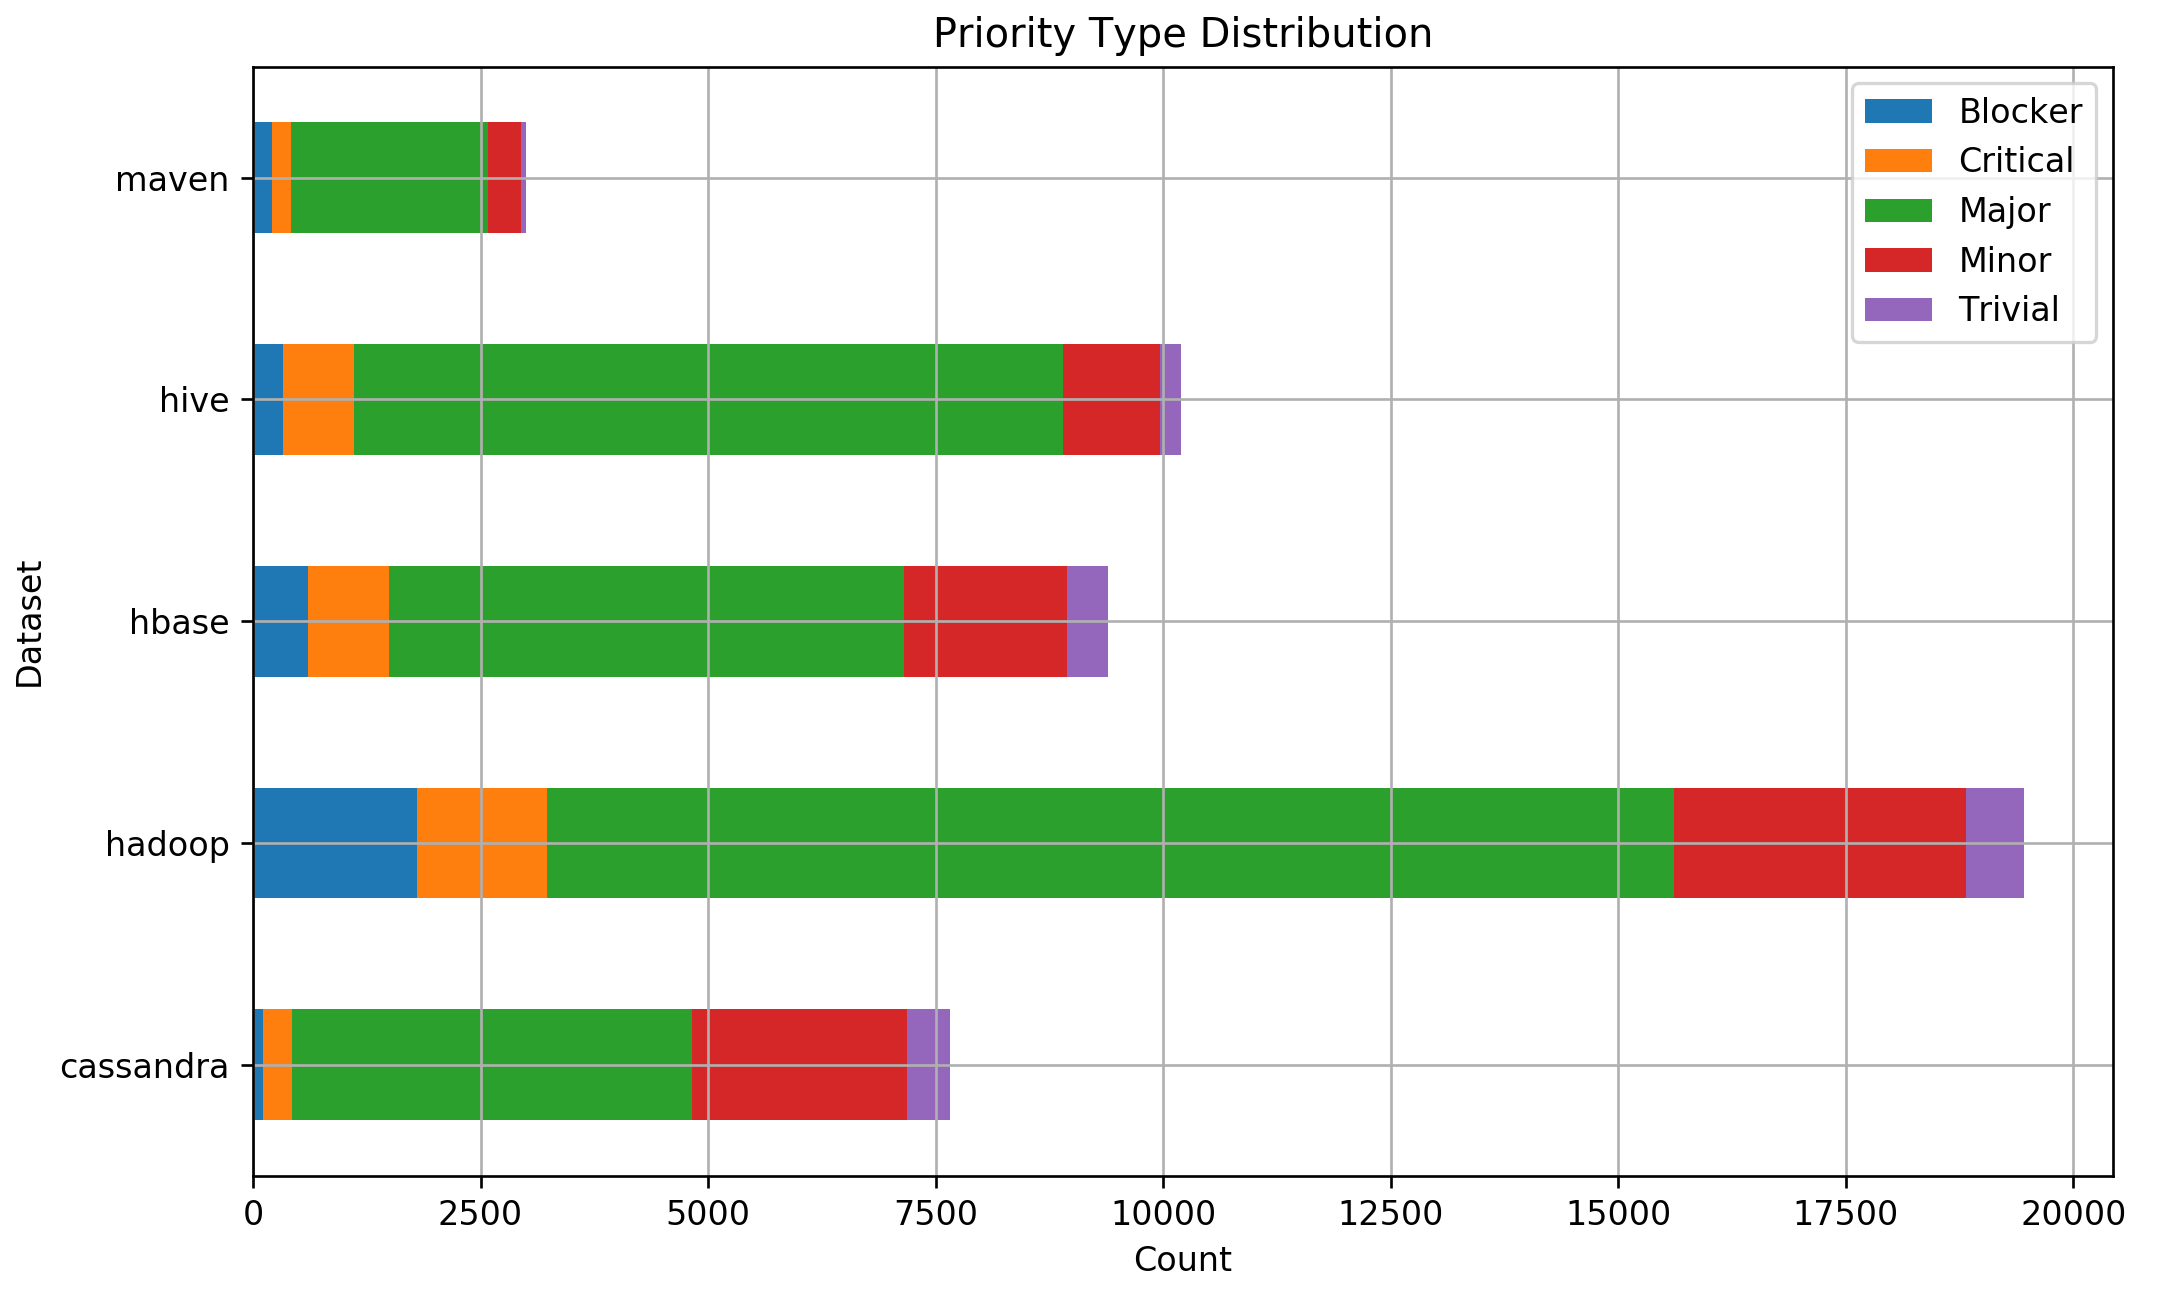
\includegraphics[width=\linewidth]{figure/prior.png}
  \caption{Count of different priority for each project}
  \label{fig:prior}
\end{figure}

More selection characteristics can be found in chapter 2.1 \cite{SEOSS33}.\\
Is fundamental to understand the structure of this dataset, the majority of the forecasting operation tests are conducted using the data stored by this research.\\
Each project is stored in an SQLITE file, a SQL offline database, the structure is based on the entity of the \textit{issue}, identified by a  \textit{issue\_id}, the other tables are used to link additional information, like the number of commit, the version referred, comments and others features. The figure \ref{fig:seoss33_db} show the database schema.

\begin{figure}[!ht]
  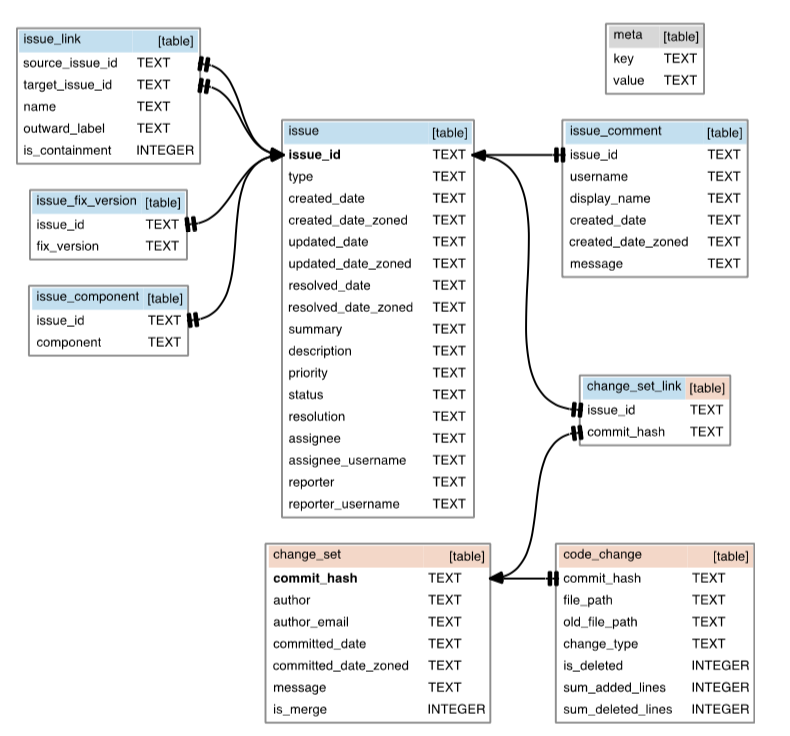
\includegraphics[width=\linewidth]{figure/seoss33_db_schema.png}
  \caption{SEOSS33 data model}
  \label{fig:seoss33_db}
\end{figure}

Each table contains different types of data that will be used to generate the data used to forecast.

% #######################################
% #          Machine Learning           #
% #######################################

\chapter{Machine Learning}
\label{chap:ml}
\section{Introduction}
Machine learning (ML) is the scientific study of algorithms and statistical models that computer systems use to perform a specific task without using explicit instructions, relying on patterns and inference instead. The word ML is almost in the public domain now, in the last decades the usage of this kind of algorithm has dramatically risen although most of it had already been developed for years. The main reason is the increase in the computational capacity of the systems.\\
There are two types of systems:
\begin{itemize}
  \item Knowledge-based: Acquisition and modeling of common-sense knowledge and expert knowledge (from rules to facts)
  \item Learning: Extraction of knowledge and rules from example/experience (from facts to rules)
\end{itemize}
All the machine learning techniques try to develop systems similar to the second definition. ML algorithms can be divided into three categories: supervised, unsupervised and reinforcement learning. The first will be used to predict class based on previous knowledge, the second tries to labeling data without a priori experience and the third bases it is learning on action reward.\\
There a lot of different models available, the following chapters will focus on the models used in this project.

\paragraph{Supervised Learning}
is a powerful technique to process labeled, which is a dataset with that has been classified, to infer a learning algorithm. This dataset is used as a basis to predict and learn how to predict unlabeled data. There are two types of supervised learning, classification, and linear regression. The goal of classification models is to predict categorical class labels of new instances, based on a training set of past observations. The classification can be binary or multi-class. Instead, regression, aim to predict continuous outcome, it tries to find mathematical relationships between variables to predict the target with a reasonable level of approximation. Our project is only focused on regression, classification will not be further discussed.

\section{Ensable Methods}
All the supervised learning method used are based on ensable, the basic idea is to merge multiple, different, hypothesis to improve the quality of the prediction, for example, the random forest or gradient boosting are ensable of multiple decision trees. The following paragraphs will deal with the models used specifically.

\paragraph{Random Forest}
Random Forest (RF) is a supervised learning algorithm that makes use of ensable learning method for classification and regression. They are built by combining the predictions of several trees, each of which is trained independently and the prediction of the trees are combined through averaging \cite{RF_theory}. A visualization of an RF is shown in figure \ref{fig:rf}.

\begin{figure}[!ht]
  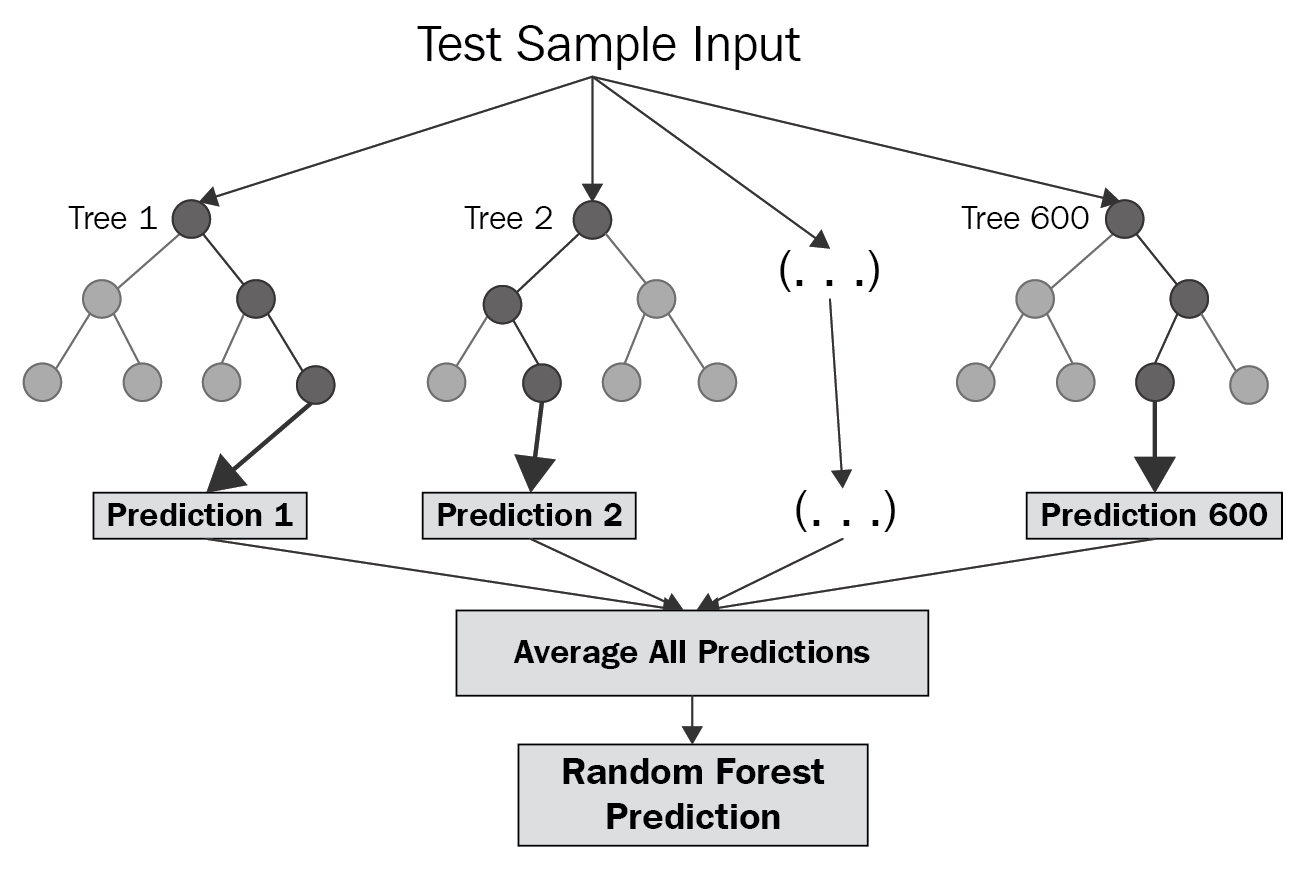
\includegraphics[width=\linewidth]{figure/rf.png}
  \caption{Random Forest simplified scheme \cite{rf}}
  \label{fig:rf}
\end{figure}

Three parameters are important to define the RF: (1) the methods for splitting the leaves, (2) the type of predictor to use in each leaf, and (3) the method for injecting randomness.
Splitting of requires the selection of shape and a method for evaluating the quality of each candidate. Typical choices are axis-aligned splits, where data is routed to sub-tree depending on a threshold. The threshold can be chosen randomly by a leaf optimization function. After the generation of different candidate splits a choosing criterion must be defined in order to split the leaf. One of the simplest strategies is to choose among the candidates uniformly at random, otherwise, it is possible to select the candidate split which optimizes a purity function (information gain for example) over the leaf that would be created.
The most common predictors, for each leaf, are the average response over training points that fall in that leaf.
The injection of randomness can happen in different ways, the size of candidate splits, coefficients for random combinations, etc\dots In any case, the thresholds can be also defined randomly or by optimization over data. Another solution is to build a tree using bootstrapped or sub-sampled dataset.\\
The training phase is performed independently by each tree by exploiting an assignment in structure and estimation points to respectively change the shape of the tree and to improve the estimator fit.\\
Once the forest has been trained it can be used to make predictions for unlabeled data points. In the prediction phase, every single tree, independently make its own prediction than an average of all the trees is computed to make a single outcome value. The contribution of each tree to the final value is the same.\\
Out implementation uses Random Forest developed by SciKit-Learn v0.21:
\begin{lstlisting}[language=python, frame=single]
  from sklearn.ensemble import RandomForestRegressor
\end{lstlisting}
The specific parameters of the model will be explained during the \autoref{chap:forecasting} about forecasting.
% To make predictions for a query point $x$, each tree independently predicts
% \begin{center}
%   \begin{equation}
%     f^{j}_{n}(x) = \frac{1}{N^{e}(A_{n}(x))} \sum_{I_{i}=e}^{Yi \in A_{n}(x)} Y_{i}
%   \end{equation}
% \end{center}
% and the forest averages the prediction of each tree
% \begin{center}
%   \begin{equation}
%     f^{(M)}_{n}(x) = \frac{1}{M} \sum_{j=1}^{M} f^{j}_{n}(x)
%   \end{equation}
% \end{center}

\paragraph{Gradient Boosting Machines}
Gradient Boosting Machines (GBM) are a family of powerful machine learning techniques that have shown considerable success in a wide range of practical applications. They are highly customizable to the particular needs of the application, line being learned with respect to different loss functions \cite{gbm}. Techniques like RF rely on simple averaging of model in the ensable. The family of boosting methods is based on a different constructive strategy of ensemble formation. Boosting add, sequentially, new models to the ensable. In GBM the learning phase consecutively fits new models to improve the accuracy of the estimations. Ideally, they construct new basic layers,  decision trees of fixed size, to be maximally correlated with the negative gradient of the loss function of the ensable. The loss function should be chosen by the developer, even ad-hoc loss function could be implemented. The attempt is to solve this minimization problem numerically via steepest descent \cite{ensable}.\\
This high flexibility of GBM makes them really customizable to any kind of task. Given its simplicity, a lot of experimentation can be performed over the model.\\
Our project implement Gradient Boosting Decision Tree (GBDT) developed by SciKit-Learn v0.21:
\begin{lstlisting}[language=Python, frame=single]
  from sklearn.ensemble import GradientBoostingRegressor
\end{lstlisting}

\section{Neural Networks}
A Neural Network (NN) is a machine learning approach inspired by the way in which the brain performs a particular learning task, network of simple computational units (neurons) connected by links (synapses). The knowledge about the learning task is given in the form of training examples, the inter neurons connection strengths (weights) are used to store the acquired information. During the learning process, the weights are modified in order to model the particular learning task correctly on the examples.\\
The learning phase can be both supervised or unsupervised. Supervised is used for pattern recognition, regression and similar is trained using data with both input and desired output. Unsupervised instead is mainly used for clustering and the learning is made using unlabeled training examples. Only supervised one will be evaluated.\\
There are three main classes of network architectures:
\begin{itemize}
  \item Single-layer feed-forward
  \item Multi-layer feed-forward
  \item Recurrent
\end{itemize}
A standard architecture is composed of three different layers, \textit{input units}, \textit{hidden units} and \textit{output units}, all the layers are linked with the learning algorithms used to train. An example of a complete multi-layer network in \ref{fig:mlff}.

\begin{figure}[!ht]
  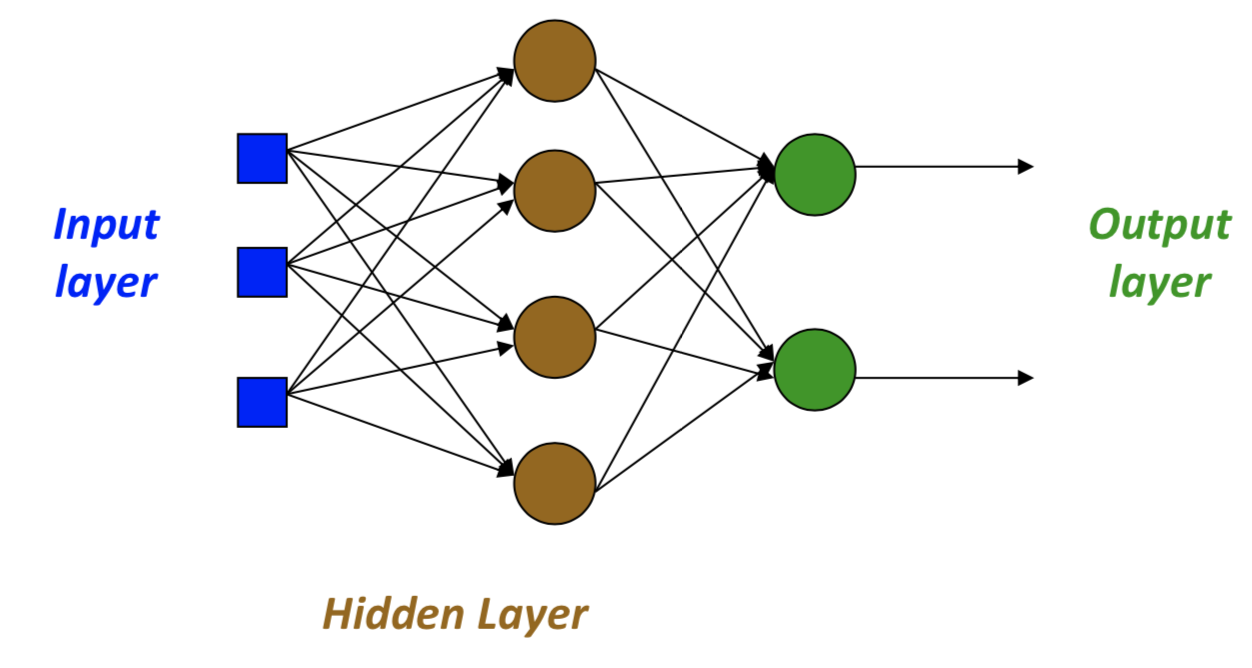
\includegraphics[width=\linewidth]{figure/feed_foward.png}
  \caption{Multi-layer feed-forward NN}
  \label{fig:mlff}
\end{figure}

The neuron is the basic processing unit of the network, which received the inputs. Each input is combined with its internal state and an optional activation function, it produces an output value that will be passed to the next layers. The weights, defined during the training phase, corresponding to the importance of the connection. The different inputs are summed using a weighted sum:
\begin{center}
  \begin{equation}
    u = \sum^{m}_{j=1} w_{j}x_{j}
  \end{equation}
\end{center}
The computed value is than scaled using an activation function $\varphi$ for limiting the amplitude of the output of the neuron by applying the function:
\begin{center}
  \begin{equation}
    y = \varphi(u + b)
  \end{equation}
\end{center}
Where $b$ represent the bias, an external parameter of the neuron, $y$ represent than the output value for the next level. An example of the structure can be found in figure \ref{fig:neuron}.

\begin{figure}[!ht]
  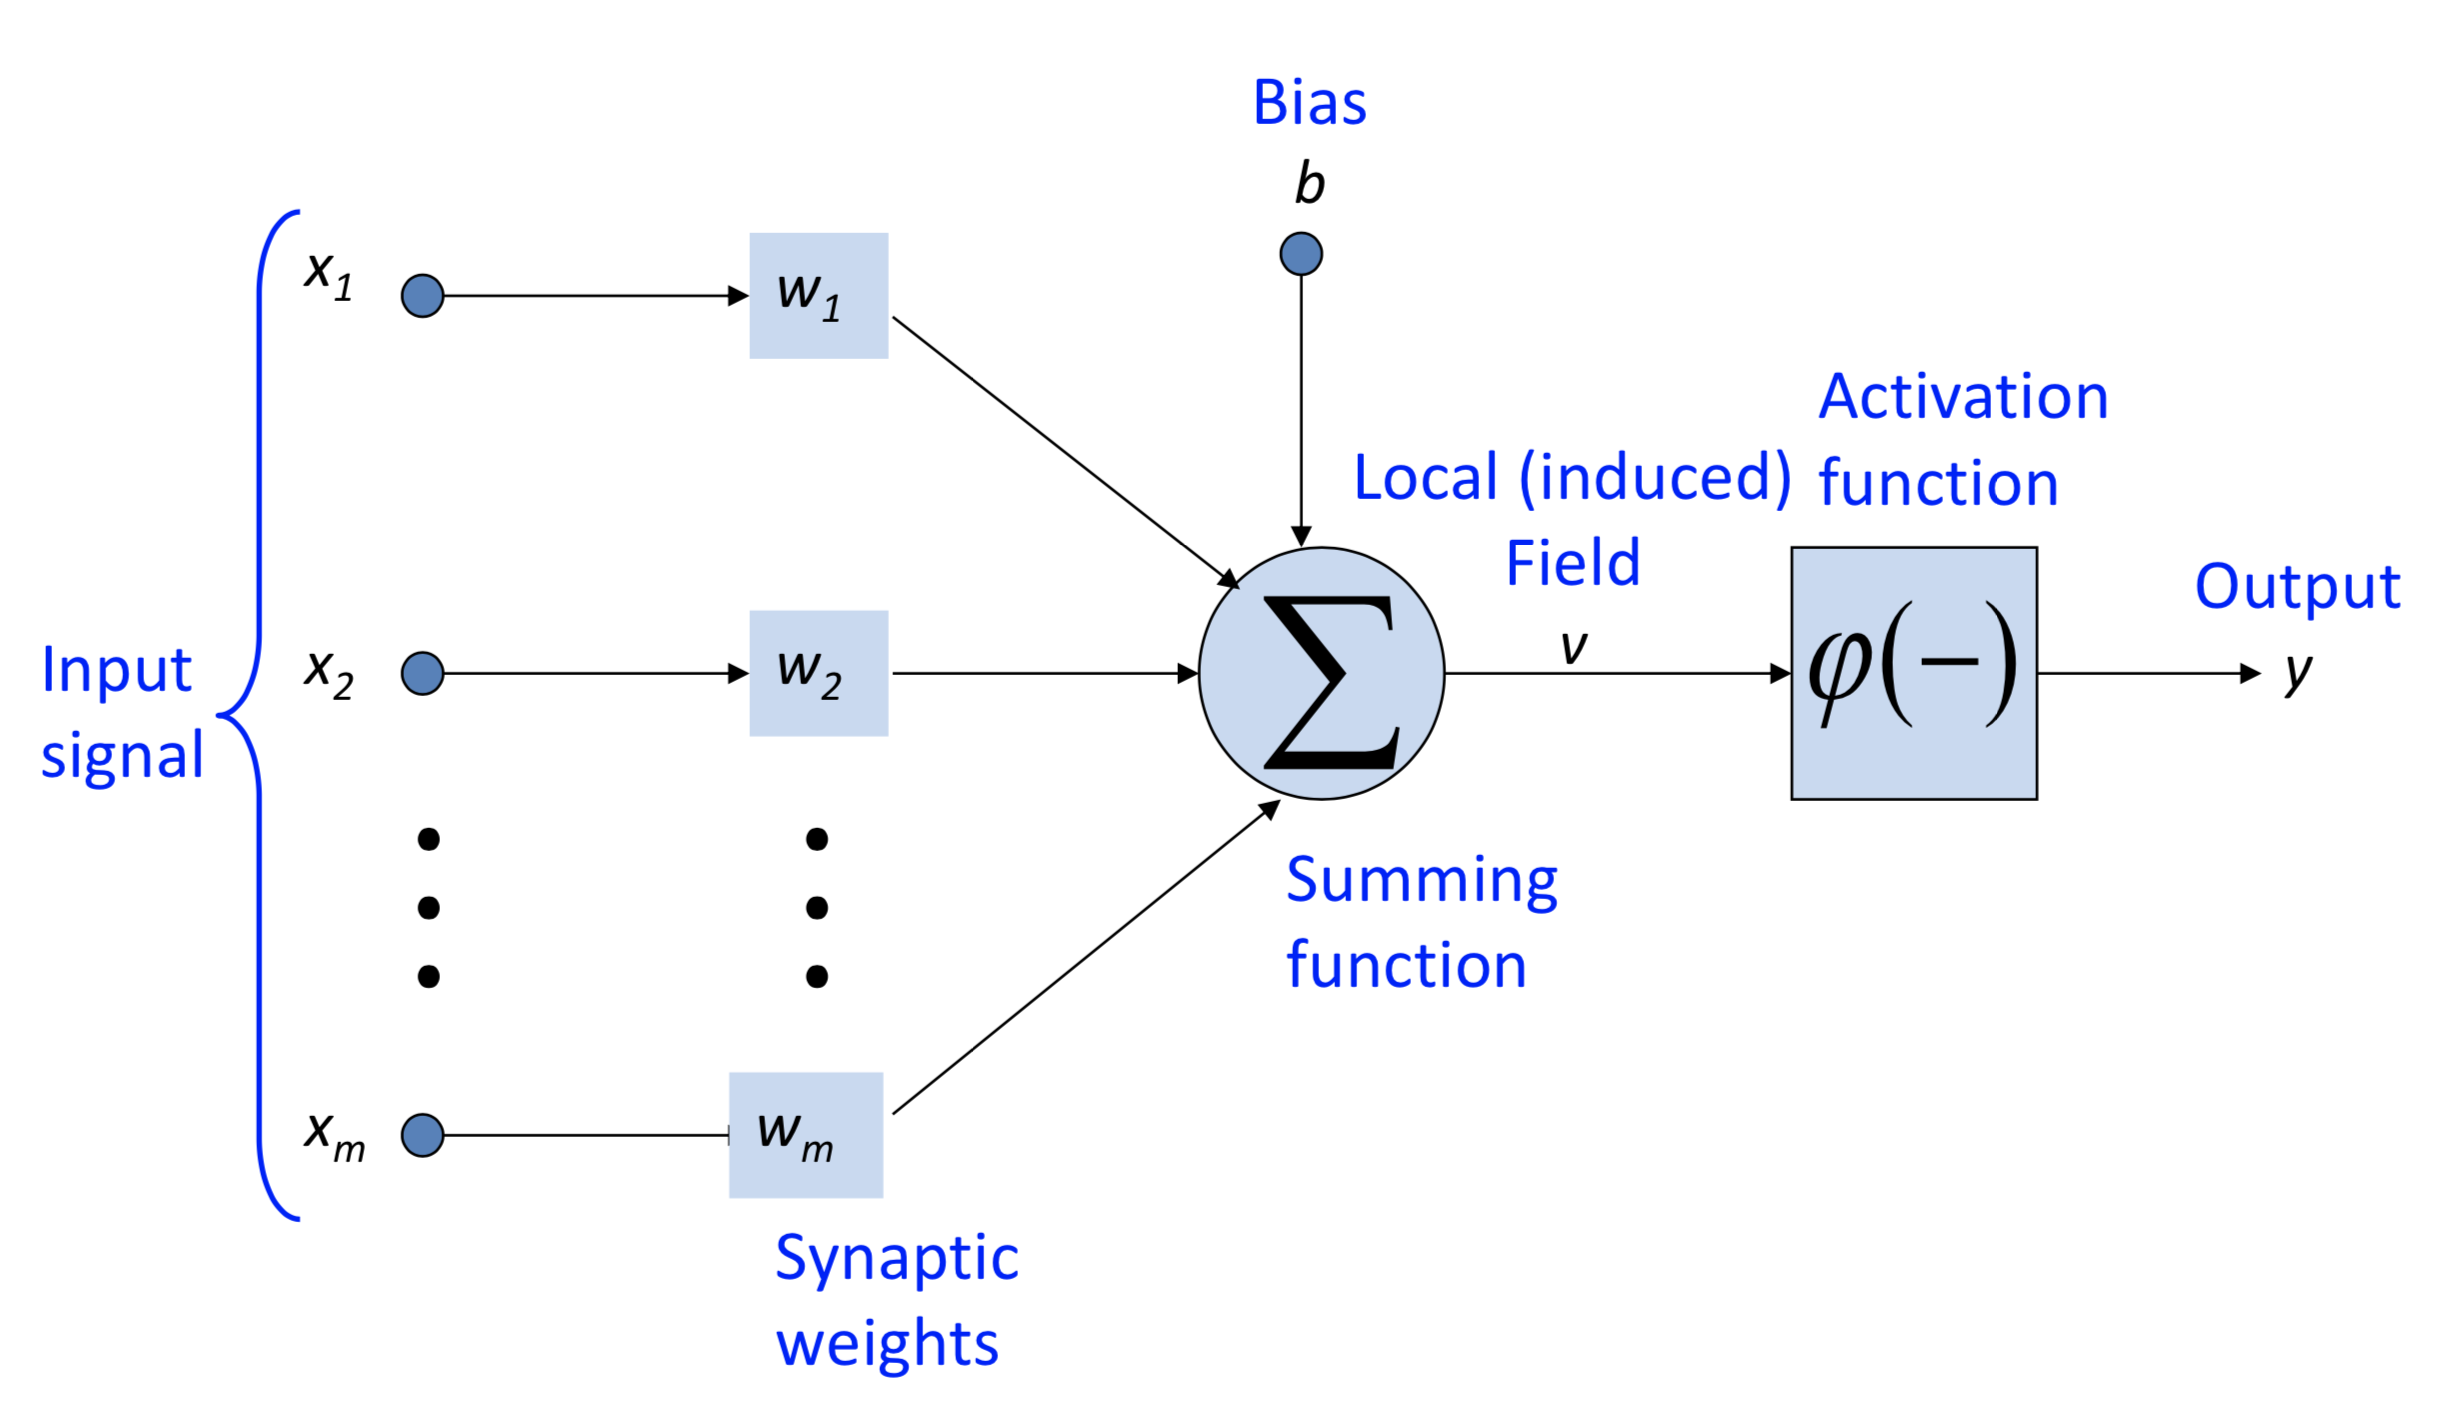
\includegraphics[width=\linewidth]{figure/neuron.png}
  \caption{Neuron view}
  \label{fig:neuron}
\end{figure}

Several different functions can be used to activate the neurons, they are trying to emulate the typical response of a biological neuron and its different activation methods. The most common are: linear, step, relu and sigmoid.
Each function behaves differently with different peculiarities and critical issues, there are two main types, linear and non-linear.

\paragraph{Step} is a binary, linear and threshold-based activation function, figure \ref{fig:step}. When the input is above or below a defined threshold, the neuron is activated and pass the same input value to the next layer. The main drawback is that not allow multiple-value output.

\paragraph{Linear} is of course a linear activation function that take the form:
\begin{center}
  \begin{equation}
    f(x) = x
  \end{equation}
\end{center}
This function takes the input and, by multiplying it by the weight of the neuron, it calculate the output. Respect the step function allows multiple-value output, but there are two major problems: it is not possible to use backpropagation (treated later) to train the network because the derivative function is constant and is not related to the input. The other problem is that linear function collapses all the layers into once because the last layer will be a linear combination of the first in any case. Figure \ref{fig:linear} show the curve.

\begin{figure}
  \centering
  \begin{minipage}{.5\textwidth}
    \centering
    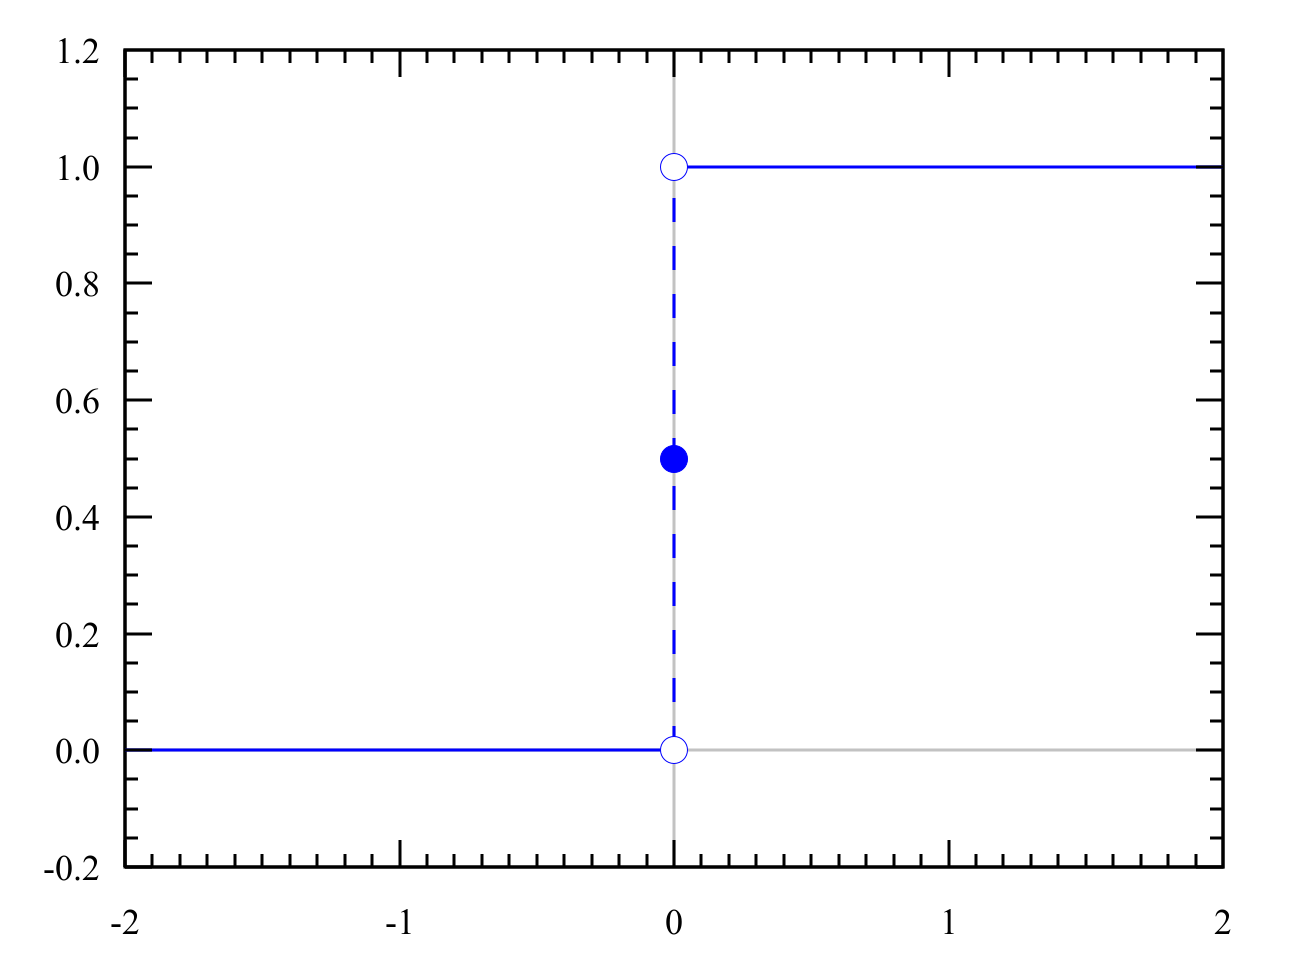
\includegraphics[width=0.85\linewidth]{figure/step.png}
    \caption{Step activation function}
    \label{fig:step}
  \end{minipage}%
  \begin{minipage}{.5\textwidth}
    \centering
    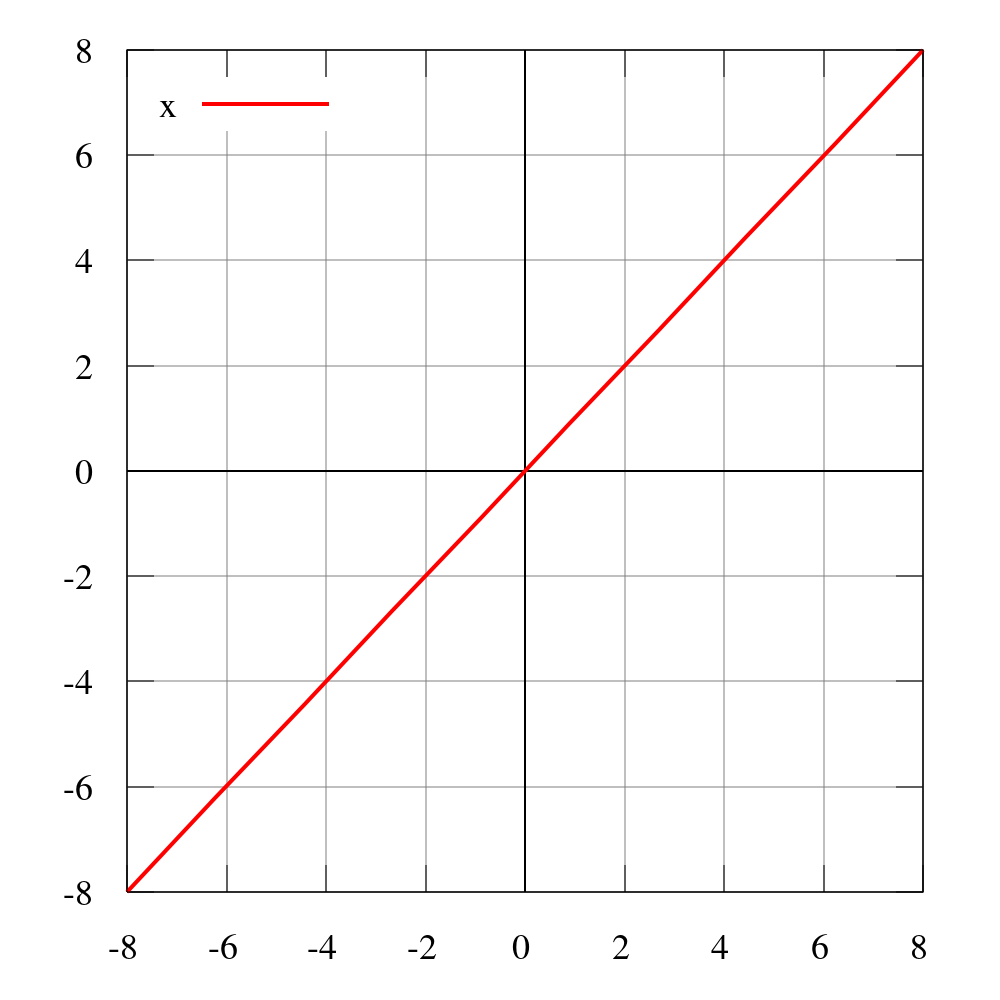
\includegraphics[width=0.75\linewidth]{figure/linear.png}
    \caption{Linear activation function}
    \label{fig:linear}
  \end{minipage}
\end{figure}

\paragraph{Sigmoid}
is a non-linear function defined in the following way:
\begin{center}
  \begin{equation}
    f(x) = \frac{1}{1+e^{x}}
  \end{equation}
\end{center}
The advantages are the smooth gradient that prevents out-of-scale output values, the implicit normalization bound from $[0, +1]$ and the cleaning of the forecast. The main drawback is the vanishing of the gradient, for very high or low input value there is no change in the prediction output, the sigmoid is also computationally expensive. The figure \ref{fig:sigmoid} show the curve.

\paragraph{ReLU} that stand for Rectified Linear Unit and is defined in the following way:
\begin{center}
  \begin{equation}
    f(x)= max(0, x)
  \end{equation}
\end{center}

Although it looks like a linear function, ReLU has a derivative function and allows for backpropagation another advantage is that is computationally efficient. The main problem of this function is its behavior with a value near zero or even negative, the gradient of the function becomes zero and the network can't perform backpropagation and can't learn.

\begin{figure}
  \centering
  \begin{minipage}{.5\textwidth}
    \centering
    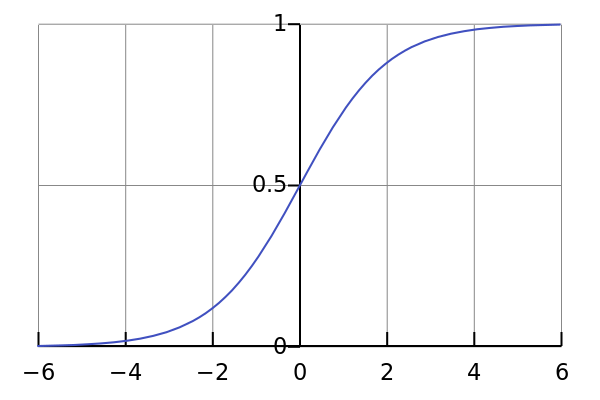
\includegraphics[width=0.8\linewidth]{figure/sigmoid.png}
    \caption{Sigmoid curve}
    \label{fig:sigmoid}
  \end{minipage}%
  \begin{minipage}{.5\textwidth}
    \centering
    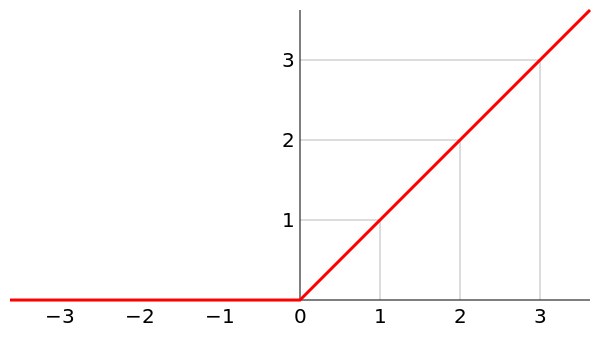
\includegraphics[width=0.8\linewidth]{figure/relu.png}
    \caption{ReLU activation function}
    \label{fig:relu}
  \end{minipage}
\end{figure}

\paragraph{Delta learning rule} uses the difference between target output and the obtained activation to drive the learning. According to these rules, each time an output is computed, the weight of the neuron is adjusted according to an error function trying to reduce the difference between output and target.

\paragraph{Backpropagation} short for \textit{"backward propagation of errors"}, is an algorithm for supervised learning of artificial neural networks using gradient descent. Given an artificial neural network and an error function, the method calculates the gradient of the error function concerning the neural network's weights. It is a generalization of the delta rule for perceptrons to multilayer feedforward neural networks. \cite{bp}.\\
The main characteristic of this technique is that the gradient, proceeds backward through the network, with the gradient of the final layer calculated before the first. This solution allows an efficient calculation of the gradient for each layer. The algorithm is structured in this form:
\begin{enumerate}
  \item Compute the error term for the output units
  \item From the output layer, repeat until last hidden reached:
  \begin{enumerate}
    \item Propagating the error term back to the previous layer
    \item Updating the weights between the two layers
  \end{enumerate}
\end{enumerate}
BP suffers the Vanishing Gradient problem, more layers are embedded in the network and more difficult become to train it. Due to the nature of the backpropagation, when an output is generated, the weight of the neurons is fixed according to the rule, each layer back the correction value is smaller, following the derivate of the activation function, in case of shallow network this problem is solved easily, for deep network this can become a real issue. The ReLU activation function manages better this problem. Another solution is the batch normalization, that rescale the input value between $[-1,1]$ in order to keep the input value far from the activation function edges. Exist a kind of network, Long Short Term Memory, developed to mitigate the vanishing gradient problem, will be discussed later.

\paragraph{Recurrent Neural Networks (RNN)}  is a class of NN that keeps connections between nodes and a temporal sequence. The main difference, respect NN, is that it has feedback connections, this memory allows us to keep track of temporal dynamic behavior, they can process a single data point or the entire sequence of data, like video or speech. They become useful as their intermediate values can store information about past inputs for a time that is not fixed a priori.\\
This kind of structures is used in a lot of different fields: image classification, captioning, sentiment analysis, machine translation, video classification, etc\dots

\paragraph{Long Short Term Memory (LSTM)} normal recurrent neural networks can connect short term event with the present, this feature can be useful in some case, another context could require more long term connection, this special RNN can handle this sort of correlations. Sometimes the recent information is enough to perform the present task, for example, trying to predict the last word of a sentence like "Sun bright in the \textit{sky}" the previous words are enough to correctly predict the last one, no more context is required. In case of more complex sentences some additional information is needed, for the phrase: "I was born in Italy and I speak \textit{italian}" the context becomes fundamental to solve the problem. In this kind of problem LSTM can be really helpful.\\
LSTM are a special kind of RNN, they were introduced by Hochreiter \& Schmidhuber (1997) \cite{lstm} and later studied and improved. It works really well on a large variety of problems. The special kind of network is explicitly designed for long term connections.
The structure of a RNN is normally a single layer, in case of LSTM the structure is more complicated, is made upon four different layers, as shown in figure \ref{fig:lstm}.

\begin{figure}[!ht]
  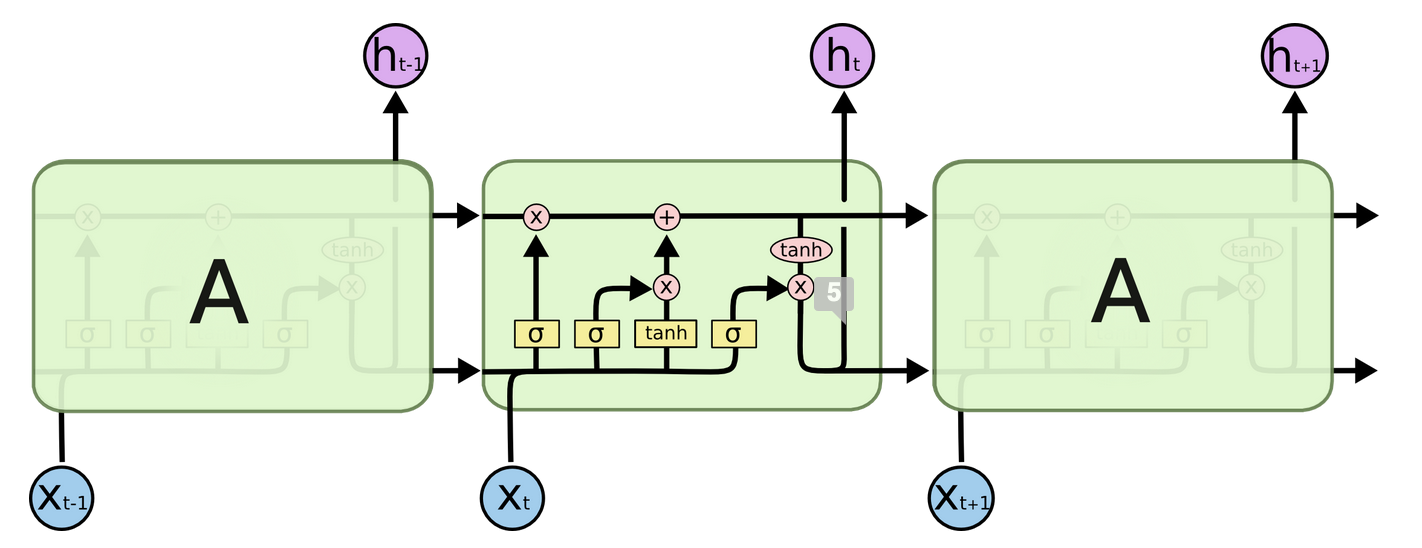
\includegraphics[width=\linewidth]{figure/lstm.png}
  \caption{Long Short Term Memory layout \cite{lstm_image}}
  \label{fig:lstm}
\end{figure}

The first layer filter the input and select what keep and not keep, the second layer will manage what information store in the cell state. The third state is in charge of update the state based on the previous step. The last one decide the output.


\section{Evaluation metrics}
Every model developed need to be evaluated, there are a lot of different methods that can be used to get metrics about the quality of the system behavior. The computation of these values is achieved via mathematical expression, for this reason, the results, are not always human-readable, some errors like mean absolute error, mean relative error and similar can be read and interpreted without any problem. For metrics like R2 or mean squared error the task becomes more complicated. The following is about the mathematical analysis and description of the different metrics used.\\
Most of metrics directly derive from the calculation of the simplest error, the \textit{absolute error}, the difference between the target $y$ and the prediction $x$:
\begin{center}
  \begin{equation}
    \epsilon = |y - x|
  \end{equation}
\end{center}
Besides being the easiest to calculate is also the easiest to be understand because show directly the distance respect the desired value.\\
The first metric based on the previous metric is the \textit{relative error}, that is computed dividing the absolute error by the target value:
\begin{center}
  \begin{equation}
    \eta = \frac{\epsilon}{|x|} = \frac{|y - x|}{|x|}
  \end{equation}
\end{center}
This error rescale the output between [0,1] in order to better understand the error in the estimation.
For example, in case of a value target value of 530 and a prediciton value of 570 the two error are:
\begin{center}
  \begin{equation}
      \epsilon = |520-570| = 50
  \end{equation}
  \begin{equation}
      \eta = \frac{50}{|520|} = 0.09
  \end{equation}
\end{center}
the difference was 50, but respect the expected output di difference is really low, around 9\%.\\
The previous errors are the basic ones, the following is the first based on aggregation of multiple errors calculation. The aggregation is fundamental to generate a single number to evaluate the quality of prediction of our model.\\
The \textit{Mean Absolute Error} (MAE), is probably the easiest to be calculated and understand, is basically computed by calculating the average of all the absolute errors:

\begin{center}
  \begin{equation}
    MAE = \frac{\sum_{i=1}^{n}{|y_{i} - x_{i}|}}{n} = \frac{\epsilon}{n}
  \end{equation}
\end{center}


% #######################################
% #             Forecasting             #
% #######################################

\chapter{Forecasting}
\label{chap:forecasting}
% \section{Introduction}
% Forecasting is the process of making predictions of future based on past and present data by trends analysis. Forecasting is one of the most desired machine learning functionality, it could be used to improve each kind of process, from finacials to production ones. Of course this task is not easy to achieve, a lot of resources and studies are needed to accomplish it.
% The software development is identical to a product development process, starts from the ideation and ends with the production itself.
% The goal is to predict the defectiveness in order to efficently allocate the development effort.

% \section{Features}
% The main advantage, in data analysis, of machines is that they can compute a lot of different data and finding a lot of patterns and correlation that human can't find. Combine the human attitude of logical correlations and machines capacity of number analysis can drive to a powerful combination that can drastically improve the forecasting ability.
% Each artificial intelligence algorithms require a correct and properly studied data in order to perform a valuable prediction, one of the basic step is the data preparation, providing correct and organized data is fundamental to correctly fit the network over the problem.

% \section{Models detail}
% \section{One-Shot Prediction}
% \section{Recurrent forecasting}
% \section{Results}


% % #######################################
% % #         Model abstraction           #
% % #######################################

% \chapter{Model abstraction}
% % \section{CommonDB}
% \section{SFBS and literature comparisons}
% \section{SFFD}


% #######################################
% #             Conclusion              #
% #######################################

\chapter{Conclusion}
Speaking about conclusion.


% #######################################
% #            BIBLIOGRAPHY             #
% #######################################
\bibliography{biblio}
\bibliographystyle{QUICKtran}


\end{document}
